\chapter{Methodology}

This chapter describes the way the research for the project was done. It is explained with sufficient details such that the device can be rebuilt again by anyone reading the report and having some basics understanding of electronics and embedded system programming.

%%%%%%%%%%%%%%%%%%%%%%%%%%%%%%%%%%%%%%%%%%%%%%%%%%%%%%%%%%%%%%%%%%%%%%%%%%%%%%%%%%%%
% SECTION: Outline
%%%%%%%%%%%%%%%%%%%%%%%%%%%%%%%%%%%%%%%%%%%%%%%%%%%%%%%%%%%%%%%%%%%%%%%%%%%%%%%%%%%%
\section{Outline}
The project is about the design of an embedded system capable meeting the light requirement as mentioned in \cref{introduction} while being user-friendly and personalisable to the user's content. To achieve this, two design methods were used. The spiral model was used to provide an understanding of the cycle of the ES, from the identification of the requirement to the validation of the user requirements. As for the  V-model, it was used to ensure a thorough testing of the device ensuring that all modules and system at a higher level function perfectly. \\
{\bf MENTION SPIRAL MODEL USE HERE}.\\
The first step in the development of the design consists of the understanding of the requirements presented in \cref{scope_and_limitations}.
%%%%%%%%%%%%%%%%%%%%%%%%%%%%%%%%%%%%%%%%%%%%%%%%%%%%%%%%%%%%%%%%%%%%%%%%%%%%%%%%%%%%
% SECTION: Research process 
%%%%%%%%%%%%%%%%%%%%%%%%%%%%%%%%%%%%%%%%%%%%%%%%%%%%%%%%%%%%%%%%%%%%%%%%%%%%%%%%%%%%
\section{Literature Review}
The review of research related to the internal clocks, how are their endogenous influencers and what technologies can be used to affect these clocks are made to get an understanding of the problem. This is not only limited to gathering information about the theory involved to meet the requirements but it also covers the reviews of documents and articles on hardware and software modules and tools that could possibly be of use.\\
Below are the questions by which the literature review was driven.
\begin{enumerate}
\item What are the problems? This step consists of seeking information about sleep disorder and its causes.
\item What biological mechanisms lead to the problem? Here research papers on biological clocks and circadian clock and rhythms were analysed to see their relationship with the problem.
\item What are the characteristics of the light causing sleep disorder? When does the reception of these lights cause a problem? A this point, there was a correlation between light and sleep disorder in humans. In order to control the effect of light on patients having sleep disorders, the characteristics (wavelength, incandescence, \ldots) of the light are required.
\item What technologies can be used to mimic these light characteristics? This step involved a careful analysis of all artificial light source technologies available.
\item What device has been created to tackle the same problem? An analysis of the competitors' devices.
\item What hardware is required by the device?
\item What communication protocol is used by each hardware?
\item What software tools are available for the development of the device software?
\item What design methodology is suitable for this type of project?
\end{enumerate}

%%%%%%%%%%%%%%%%%%%%%%%%%%%%%%%%%%%%%%%%%%%%%%%%%%%%%%%%%%%%%%%%%%%%%%%%%%%%%%%%%%%%
% SECTION: Setup
%%%%%%%%%%%%%%%%%%%%%%%%%%%%%%%%%%%%%%%%%%%%%%%%%%%%%%%%%%%%%%%%%%%%%%%%%%%%%%%%%%%%
\section{Setup}
This section describes the tools to be set prior any implementation and design. The setups are divided into two sections; the hardware setup and the software setup.
\subsection{Hardware setup}
Below are all the hardware modules required for the development of the NPSC.
\subsubsection{Personal or Desktop Computer}
A computer is needed to design, program and debug the hardware. Most of the softwares run on Windows, Linux and IOS but it is recommended that a Windows computer running on windows vista minimum is used for the development of the project. 
\subsubsection{STM32F4 Discovery board}
The STM32F4 Discovery board is the evaluation board of the STM32F407VG. It has an onboard STLink debugger to facilitate the programming of the STM32F407VG and provides all the I/O pins to the microcontroller.
\subsubsection{Arduino board}
The library made for the STM32F4 are all custom made, there is a risk of being stuck with debugging these libraries as it might be thought that the modules are not working and not the libraries. Arduino boards have libraries proven to work for most of the modules used in this project. The role of this board is purely for testing the functionalities of the modules.\\
Note that the use of this board is optional. Any Arduino board can be used; however, an Arduino Uno was used in this project. 
\subsubsection{Electronic modules}
All modules mentioned in \cref{design} are required. They are all interconnected and the absence of one can cause the whole system to fail.
\subsubsection{Logic analyser}\label{logic_analyser}
A logic analyser is a tool that analyses the data coming from one of its channel based on predefined communication protocols. This is a very useful device in debugging the modules interaction with the microcontroller. The logic analyser used for this project is one of the Salea logic analysers.
\begin{figure}[ht]
\centering
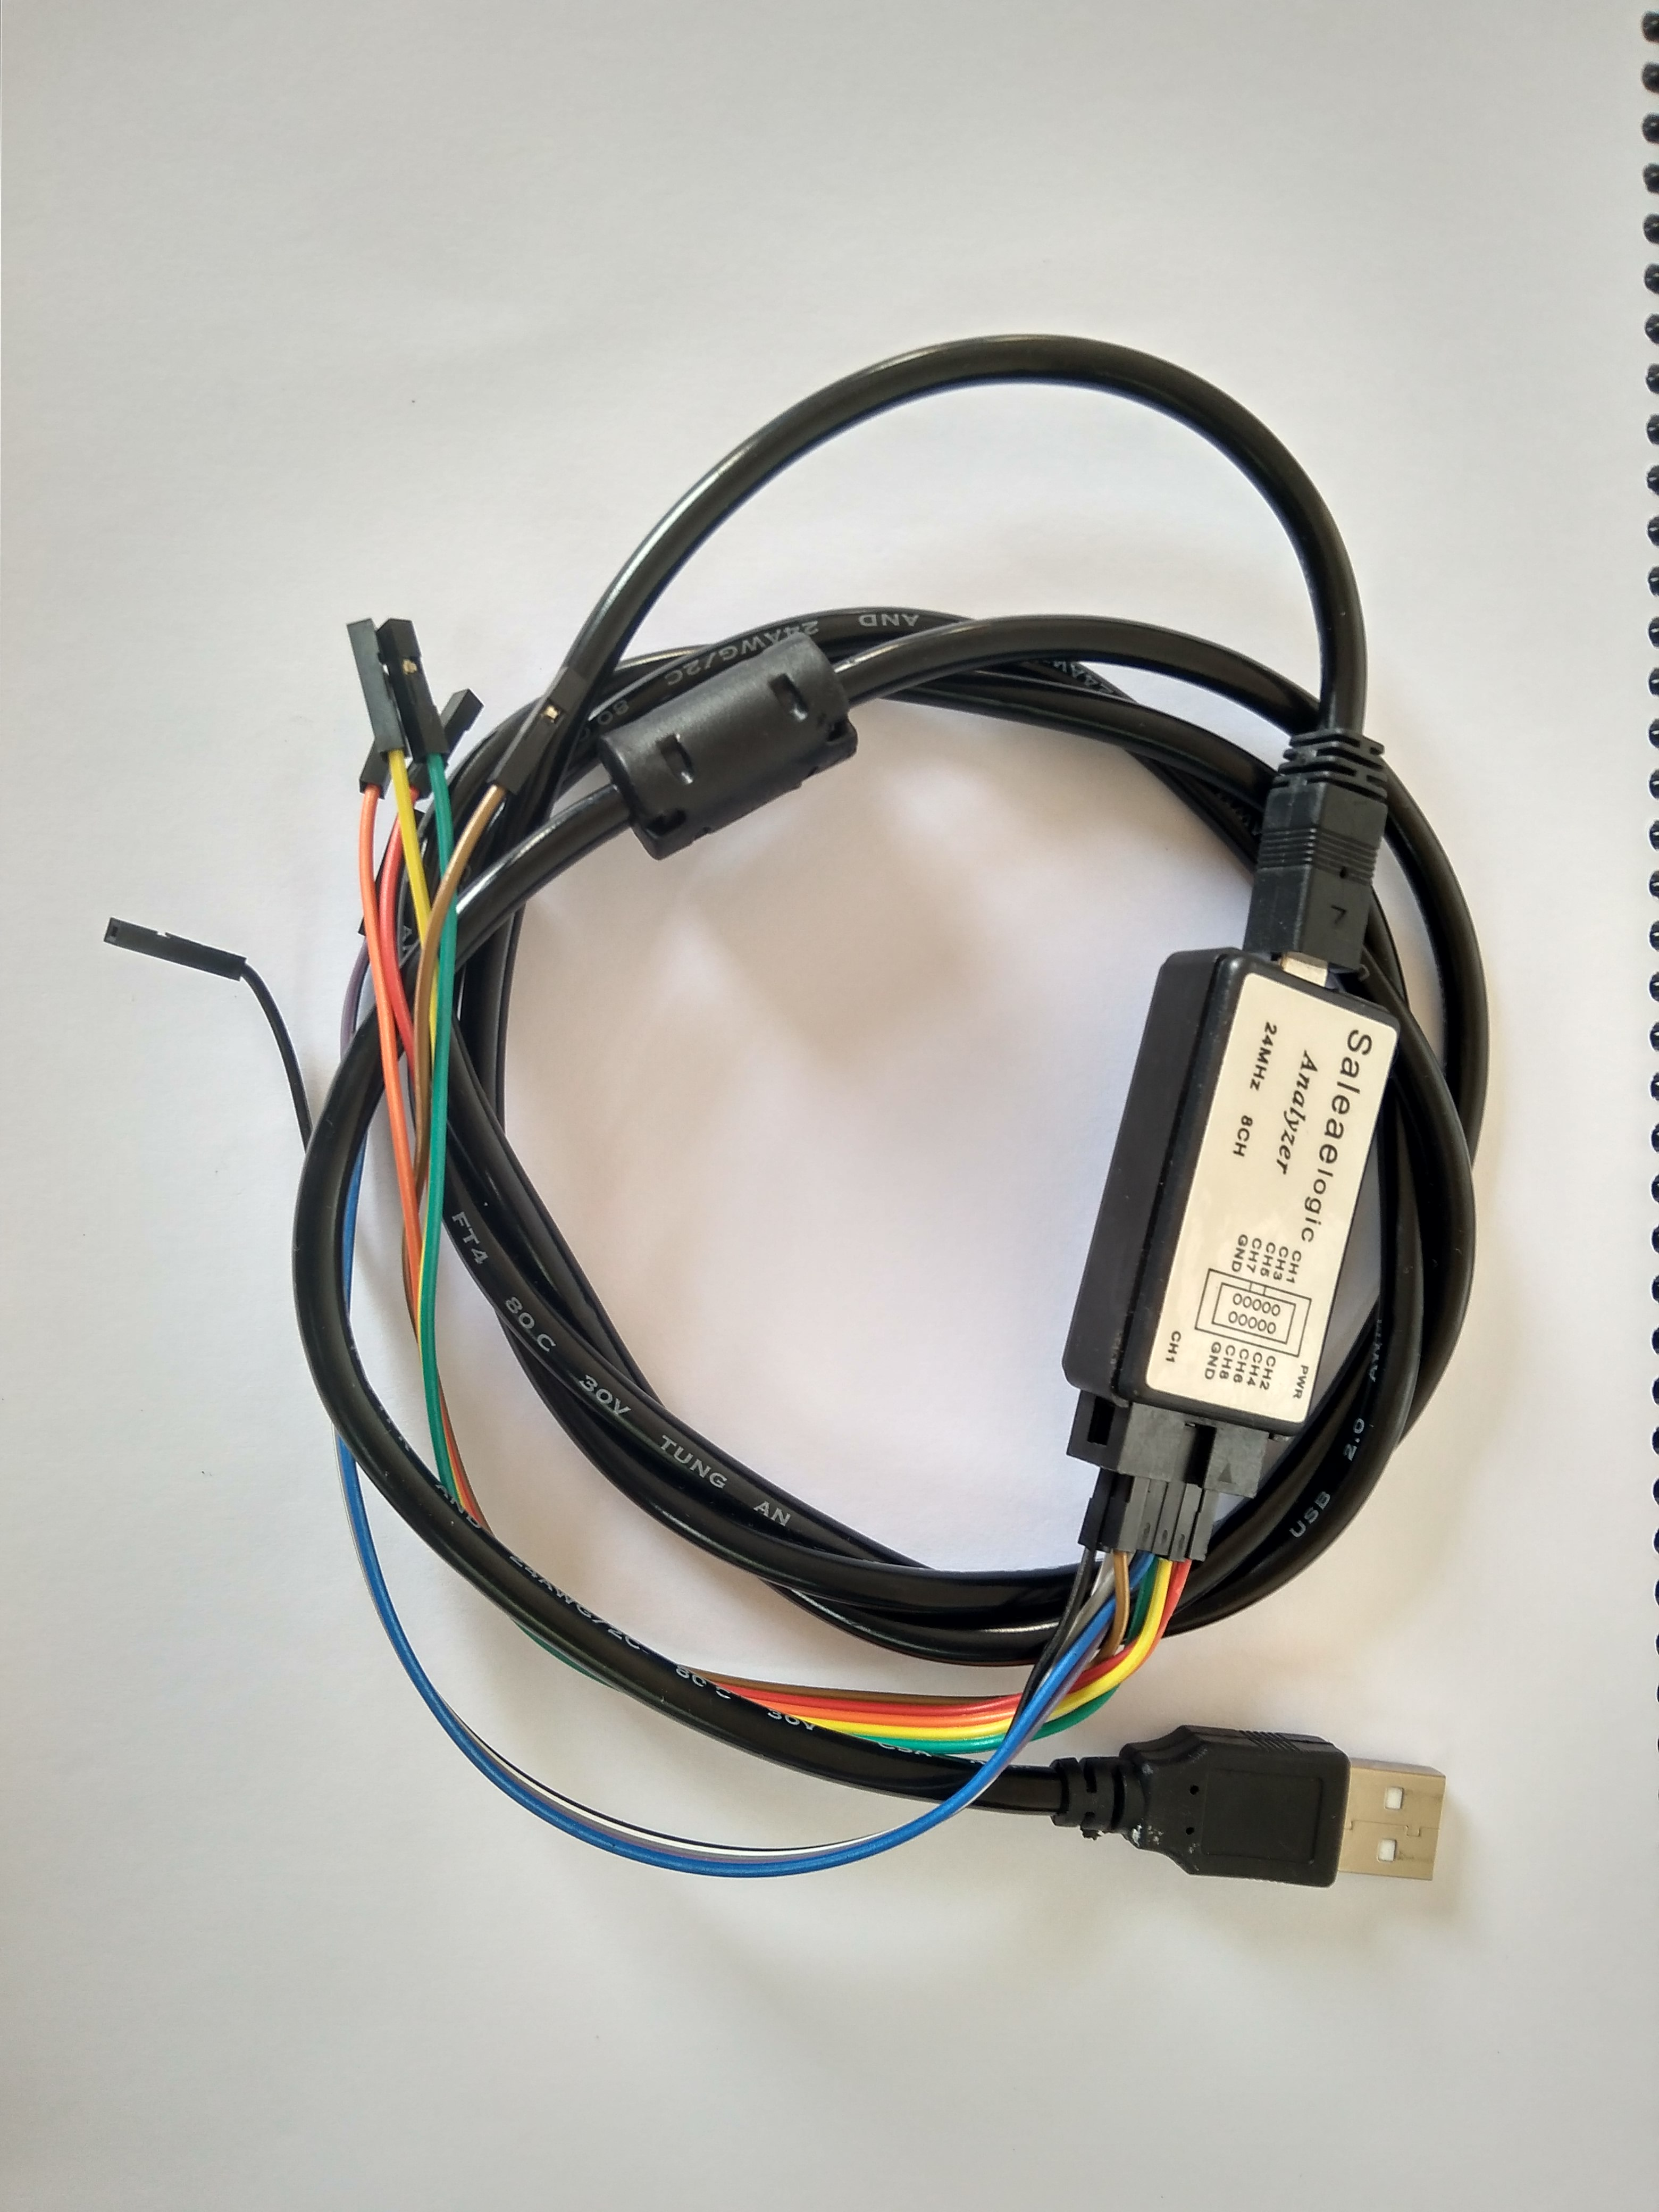
\includegraphics[scale=0.05]{logic_analyser.jpg}
\caption{Salea logic analyser.}
\label{fig:logic_analyser}
\end{figure}
\subsubsection{Serial to USB converter}
The Serial to USB converter allows the translation of UART commands to USB command. This module is required to program the Nextion screen.
 
\subsection{Software setup}
Certain software tools are required for the development of the NPSC software. Those mentioned below are the one used for this project, other version or type of software can be used as long as they have the same functionalities as the one listed below.
\subsubsection{Atolic TrueSTUDIO}
Atolic TrueSTUDIO provides debugging functionalities such as breakpoint, memory and register observation as well as backtracking. It contains all the STM libraries which facilitate development. Moreover, it comes with STLink so no external debugging setup is required. Other IDEs such as Keil or Eclipse can also be used instead of Atolic TrueSTUDIO. In such case, it is essential to make sure that C is installed as well as gdb and STlink alongside its drivers. 
\subsubsection{Nextion IDE}
The Nextion IDE is the only IDE capable of programming the Nextion TFT touchscreen and only runs on windows. It provides a Graphical User Interface when visual components can be dragged to the screen. Each type of component has specific parameters and events. The IDE also allows the user to program the behaviour of a component depending on its events. Before uploading the program to the Nextion screen, the user should use the debugging mode to test the logical behaviour implemented and the data transfer of the screen.    
\subsubsection{Logic analyser software}
The logic analyser mentioned in \cref{logic_analyser} requires the use of the Salea software which runs on Windows, Linux and IOS. The software allows the selection of up to eight channels whose data can be visualised and analysed. Before analysing the data, the sampling rate and time period must be set based on the baud rate or frequency of the pin to debug. After the first setup, an analyser is set up to the desired communication protocol. In this project only the protocols mentioned in \cref{com_protocols} are needed. The data can be collected and automatically analysed once the setup stage is done.
 \subsubsection{PCB design software: Altium Designer}
A PCB design software is required in the design of the hardware. The one used for this project is Altium designer as the university has a working license and Altium has more sophisticated features than its competitors. 
\subsubsection{API generator: Doxygen}
The interactions between the elements in the system become more complex for every hardware module, sub-system and system design added to the project. In order to keep track of these interactions, an API generator is required. An API generator generates the documentation of the system based on the comments in each file. Doxygen which is popular among the API generator, especially for ES is used for this project.
\subsubsection{Version Control: git}
The whole project is under a version controller. Each implementation type (hardware, software, report, mechanical, \ldots) has its own branch to control each change made in the project. This project repository is under git and can be found on \href{https://github.com/Kojey/NPSC}{github.com}. 
%%%%%%%%%%%%%%%%%%%%%%%%%%%%%%%%%%%%%%%%%%%%%%%%%%%%%%%%%%%%%%%%%%%%%%%%%%%%%%%%%%%%
% SECTION: Implementation
%%%%%%%%%%%%%%%%%%%%%%%%%%%%%%%%%%%%%%%%%%%%%%%%%%%%%%%%%%%%%%%%%%%%%%%%%%%%%%%%%%%%
\section{Implementation}
The NPSC requires hardware and software modules. For the first prototype, certain hardware modules off the shelves can be used, as for other modules, they require to be designed and manufactured as modules with their specific characteristics do not exists on the market.\\
The implementation was broken into two main sections, the hardware implementation and the software implementation. The software implementation relies on the functioning of the hardware. To ensure that the system is implemented in a way that uses the time efficiently, it was implemented following the hierarchy illustrated in \cref{fig:system_hierarchy}. 
\begin{figure}[ht]
\centering
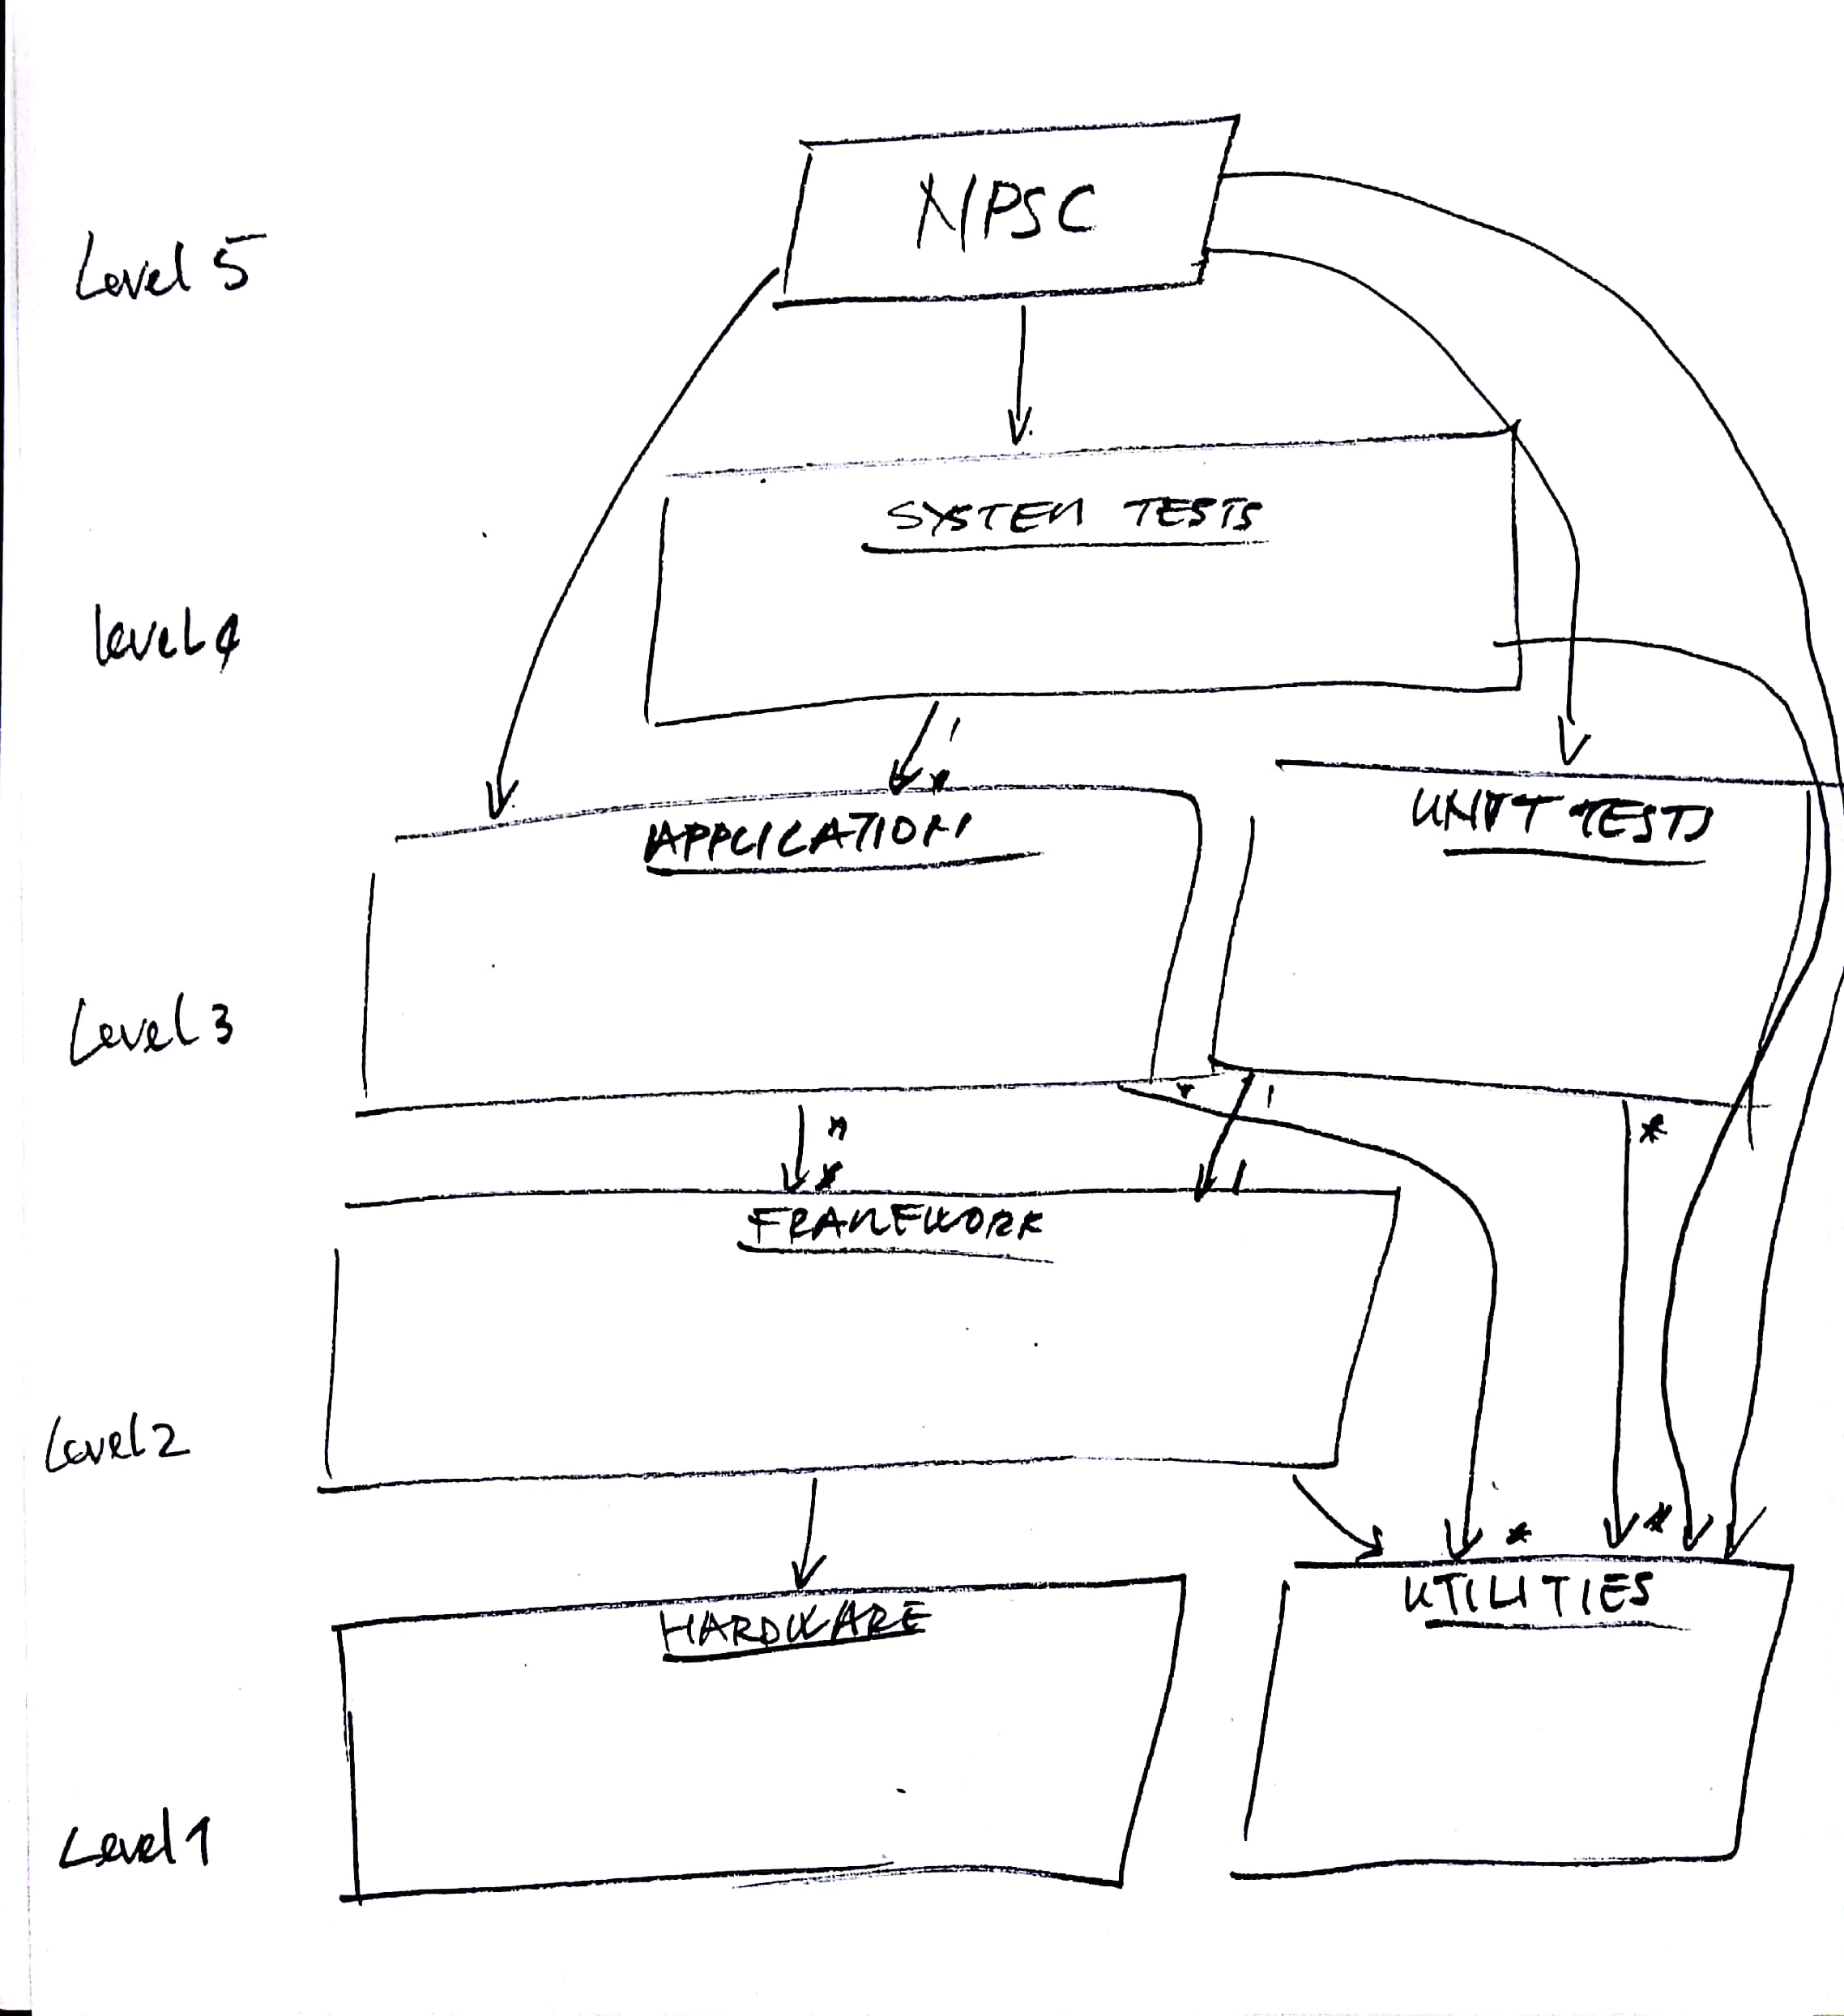
\includegraphics[scale=0.15]{system_hierarchy.jpg}
\caption{Overview of the implementation hierarchy. Implementation starts from the bottom with the collection or design and manufacturing of the hardware followed by the software implementation}
\label{fig:system_hierarchy}
\end{figure}
\Cref{fig:system_hierarchy} has five levels. Elements from the same level are able to call functions of the level below and not vice-versa. This implies that in order to implement one level, the level bellow must exist and function. The levels and their interactions are details as follow:
\subsection{Level 1: Hardware and Utilities}  
The hardware and the utilities software are at the bottom of the hierarchy and are the first to be implemented. The hardware is manufactured and assembled, as for the off the shelves modules, a basic test using the Arduino is performed on the modules. The utilities software contains all the common functionalities or structures required by the element at higher levels. This element might not be implemented initially, in reality, this element is continuously modified based on the need of the higher elements.
\subsection{Level 2: Framework}   
The framework element contains all the framework required by each hardware module. There is a one-to-one relationship between the framework modules and the hardware modules. The framework provides the basic functions required by higher modules. For example, each framework module provides an initialization function used to initialised the communication between its corresponding hardware module and the NPSC. 
\subsection{Level 3: Application and Unit tests}   
The unit test provides tests for each framework module. There is also a  one-to-one relationship between the unit test modules and the software modules. The application element of the hierarchy contains all application codes required by the system. These applications have a one-to-many relationship between them and the framework modules. For example, the alarm application requires the internal RTC framework and the external RTC framework. 
\subsection{Level 4: System tests}   
The system tests contain the test designed to verify the system requirements. An example of a test is checking that a specific command from the screen executes the right command.
\subsection{Level 5: NPSC}   
The NPSC is the highest level of the hierarchy. It, however, existed since the first implementation of the framework. It is used to call all the function needed for the application element and to run the unit and system tests.

%%%%%%%%%%%%%%%%%%%%%%%%%%%%%%%%%%%%%%%%%%%%%%%%%%%%%%%%%%%%%%%%%%%%%%%%%%%%%%%%%%%%
% SECTION: Experimentation
%%%%%%%%%%%%%%%%%%%%%%%%%%%%%%%%%%%%%%%%%%%%%%%%%%%%%%%%%%%%%%%%%%%%%%%%%%%%%%%%%%%%
\section{Experimentation}
This section presents the different tests designed to ensure that each hardware modules, sub-systems and system requirements are met. Each experiment targets one specific element from the hierarchy in \cref{fig:system_hierarchy}.
\subsection{Hardware tests}
The hardware testing requires careful test are any wrong connection could possibly damage the hardware. Two main tests are made on the hardware, a basic test testing the functionality of the hardware modules and the neopixel ring PCB test to ensure that the light requirement is met.
\subsubsection{Basic hardware test}\label{basic_hardware_test}
Most hardware communicates to the microcontroller through the protocols mentioned in \ref{com_protocols}. The test of these hardware is done using these steps:
\begin{enumerate}
\item Check connection to the micro using the hardware datasheets
\item Check power connections
\item Check functionality of module using benchmark testing (Arduino) if available otherwise use framework module to test hardware \footnote{Is it risky to use the framework module to test the hardware as it has not been tested at this stage}
\item Use Salea logic analyser to verify the data received from the hardware is correct.
\end{enumerate} 
\subsubsection{Neopixel ring test}
The Neopixel ring has light and current requirements. The light requirement is tested using a lux meter available in smartphones. As for the current requirement, the current withdrawn by the PCB is measure are different light intensity. 

\subsection{Software tests}
The software tests rely on the hardware, therefore, the hardware tests must be run prior these tests. There are two types of test performed, namely the communication protocol tests (coms tests) and the logic tests.\\
The coms tests are performed using the debugging tools of the selected IDE (Atolic TrueSTUDIO in this project). Breakpoints are used alongside the Salea logic analyser to verify the information transferred between the STM32F4 and the hardware modules.\\
The logic tests are performed during runtime or using the IDE debugger \footnote{The IDE debugger is done to pinpoint the point of failure in the code. It might require the use of a com test and is used if the runtime test fails}. The logic tests make use of a visual signal (either via the Nextion screen or Android application or Neopixel ring) to output the outcome of the tests.\\
There are two levels of software tests, the unit tests and the system tests.
\subsubsection{Unit tests}
Unit tests are designed to test the framework of the hardware modules. These tests are logic tests performed on the hardware. One example of these test is verifying the data stored on the storage after a write operation, or getting the colour from one neopixel. Unit tests also include indirect hardware interaction functions such as functions which convert a structure of data into another. 
\subsubsection{Integrations tests}
Systems tests are at a higher level than the unit tests. They are all logic tests ensuring that the interaction between the framework modules is as expected. When these tests fail, the unit tests of the involved framework modules must be tested. If the unit tests pass, it is certainly a logic error and the IDE debugger must be used to pinpoint the errors.

\subsection{Performance tests}
This tests gather data on the performance of each module and of the system as a whole. It is meant to answer the following question:
\begin{enumerate}
\item What is the optimal queue size for the instruction buffer?
\item What is the optimal DMA size for each input? 
\end{enumerate} 
\subsection{Acceptance tests}
This is the final test done to prove that the device meets all the requirements defined in \cref{scope_and_limitations}. This test involves using the device as a user and verify the functionalities of the device. 
%%%%%%%%%%%%%%%%%%%%%%%%%%%%%%%%%%%%%%%%%%%%%%%%%%%%%%%%%%%%%%%%%%%%%%%%%%%%%%%%%%%%
% SECTION: Analysis
%%%%%%%%%%%%%%%%%%%%%%%%%%%%%%%%%%%%%%%%%%%%%%%%%%%%%%%%%%%%%%%%%%%%%%%%%%%%%%%%%%%%
\section{Analysis}
This section provides analysis of the tests performed during the experiments. 
{\bf TODO}
